\documentclass{standalone}
\usepackage[margin=1in,vmargin=1in]{geometry}
\usepackage{tikz}
\usepackage{graphicx}

\begin{document}
\newcommand\myopacity{0.4}
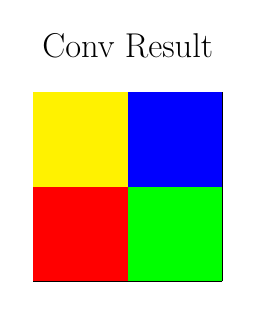
\begin{tikzpicture}[thick,scale=0.6, every node/.style={scale=0.6}]
  % -=-=-=-=- RESULTING IMAGE -=-=-=-=-
  \node(text) at (2,5) {\huge{Conv Result}};
  \node (A) at (0,0) {};
  \node (B) at (4,4) {};
  \draw[step=1cm,black,thin] (A) grid (B);
  \node (a) at (0.5,0.5) {\Huge{$0$}};
  \node (b) at (1.5,0.5) {\Huge{$0$}};
  \node (c) at (2.5,0.5) {\Huge{$2$}};
  \node (d) at (3.5,0.5) {\Huge{$0$}};

  \node (e) at (0.5,1.5) {\Huge{$0$}};
  \node (f) at (1.5,1.5) {\Huge{$4$}};
  \node (g) at (2.5,1.5) {\Huge{$6$}};
  \node (h) at (3.5,1.5) {\Huge{$0$}};

  \node (i) at (0.5,2.5) {\Huge{$0$}};
  \node (j) at (1.5,2.5) {\Huge{$4$}};
  \node (k) at (2.5,2.5) {\Huge{$5$}};
  \node (l) at (3.5,2.5) {\Huge{$0$}};

  \node (m) at (0.5,3.5) {\Huge{$0$}};
  \node (n) at (1.5,3.5) {\Huge{$4$}};
  \node (o) at (2.5,3.5) {\Huge{$3$}};
  \node (p) at (3.5,3.5) {\Huge{$0$}};

  \fill[red,opacity=\myopacity] (0,0) rectangle (2,2) {};
  \fill[yellow,opacity=\myopacity] (0,2) rectangle (2,4) {};
  \fill[green,opacity=\myopacity] (2,0) rectangle (4,2) {};
  \fill[blue,opacity=\myopacity] (2,2) rectangle (4,4) {};
\end{tikzpicture}\hspace{0.75cm}
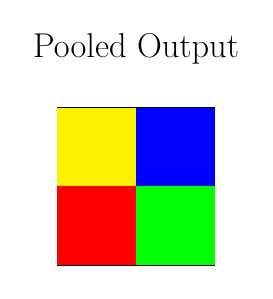
\begin{tikzpicture}[thick,scale=1, every node/.style={scale=0.6}]
  % -=-=-=-=- RESULTING IMAGE -=-=-=-=-
  \node(text) at (2,3.75) {\huge{Pooled Output}};
  \node (A) at (1,1) {};
  \node (B) at (3,3) {};
  \draw[step=1cm,black,thin] (A) grid (B);
  \draw[black,thin] (1,1) -- (3,1);
  \draw[black,thin] (1,1) -- (1,3);

  \node (a) at (1.5,1.5) {\Huge{$4$}};
  \node (b) at (2.5,1.5) {\Huge{$6$}};
  \node (c) at (1.5,2.5) {\Huge{$4$}};
  \node (d) at (2.5,2.5) {\Huge{$5$}};

  \fill[red,opacity=\myopacity] (1,1) rectangle (2,2) {};
  \fill[yellow,opacity=\myopacity] (1,2) rectangle (2,3) {};
  \fill[green,opacity=\myopacity] (2,1) rectangle (3,2) {};
  \fill[blue,opacity=\myopacity] (2,2) rectangle (3,3) {};
\end{tikzpicture}
\end{document}